\section{摩擦起电的原因}\label{sec:7-2}

我们从化学课里已经知道,有些物质是直接由原子构成的,有些物质是由分子构成的,而分子也是由原子构成的。
原子的中心是由带正电的质子和不带电的中子组成的原子核,核的周围是高速运动的带负电的电子。
在通常情况下,原子核带的正电跟核外电子总共带的负电数量相等,整个原子是中性的。
图 \ref{fig:7-6} 是氢、氦、锂的原子结构的模型。

\begin{figure}[htbp]
    \centering
    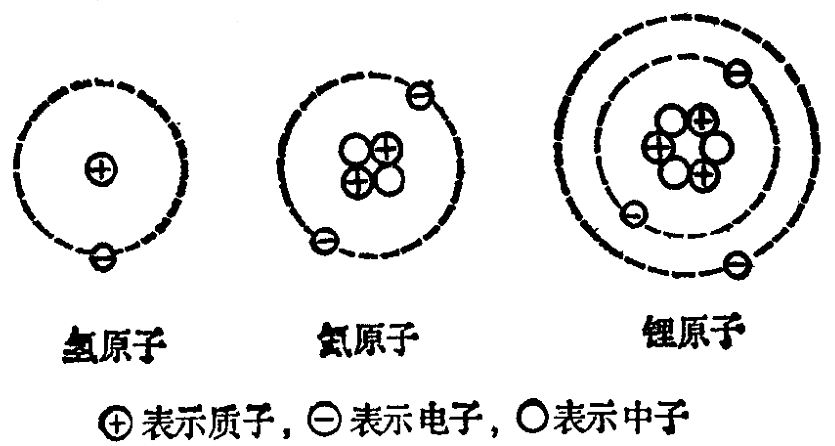
\includegraphics[width=0.6\textwidth]{../pic/czwl2-ch7-6}
    \caption{氢、氦、锂的原子结构模型}\label{fig:7-6}
\end{figure}

本来是中性的原子,当它失去一个或几个电子的时候,它的电子总共带的负电数量比原子核的正电少,它就显示出带正电;我们称它为正离子。
相反,本来是中性的原子,当它跟多余的电子结合在一起的时候,它就显示出带负电;我们称它为负离子。

在通常情况下,由于原子是中性的,因而物体也呈中性。
那么,当两个物体相互摩擦的时候,为什么物体能带电呢?
原来,不同物质的原子核束缚电子的本领不同。
当两个物体相互摩擦的时候,哪个物体的原子核束缚电子的本领较弱,它的一些电子就会转移到另一个物体上。
失去电子的物体因缺少电子而带正电,得到电子的物体则因有了多余电子而带等量的负电。
例如玻璃跟绸子摩擦,玻璃的一些电子转移到绸子上,玻璃因失去电子而带正电,绸子因得到电子而带等量的负电。
橡胶跟毛皮摩擦,毛皮的一些电子转移到橡胶上,橡胶带负电,毛皮带等量的正电。

可见,摩擦起电并不是创造了电,只是电子从一个物体转移到另一个物体。

我们如果让两个带等量的异种电荷的物体互相接触,带负电的物体上多余的电子转移到带正电的物体上,
那么,这两个物体都没有多余的电子,也不缺少电子,都恢复成不带电的状态。
这种现象叫做正、负电荷的中和。



\section*{阅读材料:人类对摩擦起电的认识}

摩擦起电的现象虽然发现很早,但是在长达两千多年的时间里,只停留在观察琥珀的摩檫起电上。
第一个认真研究电现象的是英国医生吉尔伯特(1540 ~ 1603),他想搞清楚琥珀为什么会有那种神奇的吸引力。
1600 年,他发现金刚石、水晶、硫磺、火漆和玻璃等物质,在用呢绒、毛皮或丝绸摩擦过后,象琥珀那样有神奇的吸引力。
这使他领悟到这种现象并不是琥珀特有的,于是他想可能一切物质中都蕴藏着一种看不见的流体,
当受到摩擦的时候从物质中被挤出来,他把这种看不见的特殊流体叫做“电"。这是对摩擦起电现象最早的猜想。

1734 年,法国化学家杜菲发现电有两种,同种电相异斥,异种电相吸。
他把这两种电分别叫“玻璃电”和“琥珀电”。
当带“玻璃电”的物体和带“琥珀电”的物体互相接触的时候,电的性质会减弱甚至消失,
象正、负数能互相抵消一样,所以美国学者富兰克林(1706~1790)把它们叫“正电”和“负电”。
1747 年富兰克林还提出一种假说,被称为“单流休说”,用来解释摩擦起电。
这种假说认为:在一切物质中都存在着一种正的“电流体”,物林中的“电流体”
比正常状态的时候多,物体就带正电,
比正常状态的时候少,物体就带负电;
两个物体互相摩擦,“电流体”从一个物体流入另一个物体,所以一个带正电,一个带负电。

1759 年,英国物理学家塞麦发展了杜菲的看法,提出了新的“双流体说”,认为一切物质中都存在两种“电流体”,
一种是正的,一种是负的;正常状态下的物体中,这两种流体的量相等,它们的作用互相抵消了。
当两个物体互相摩擦的时候,就会有流体的转移,结果,
  一个物体中的正流体超过平衡量,显示带正电,
另一个物体中的负流体超过平衡量,显示带负电。

单流体说的支持者和双流体说的支持者有过长期的争论,但是直到十九世纪末还没有令人信服的实验表明哪一个正确。
二十世纪初人类认识了原子的结构以后才知道,这两种假说都有正确的成份。
事实上,物体中既有正电荷,又有负电荷,双流体说在这一点上是正确的;
但是在摩擦起电时,只是带负电荷的电子从一个物体流入另一物体,在只是有一种电荷能够流动这一点上,单流体说是正确的。


\lianxi

\begin{wrapfigure}{r}{5cm}
    \centering
    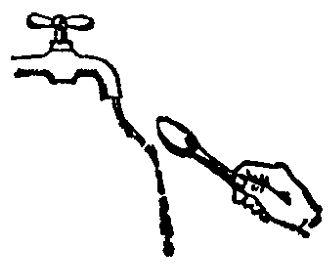
\includegraphics[width=4cm]{../pic/czwl2-ch7-7}
    \caption{}\label{fig:7-7}
\end{wrapfigure}

(1) 用什么方法可以检验出经过摩擦的物体是否带上了电?

(2) 当验电器上的金属球跟带正电的物体接触时,金属球也带上了正电。你能够解释这种现象吗?

(3) 当验电器上的金属球跟带负电的物体接触时,金属球也带上了负电。你能够解释这种现象吗?

(4) 用带电体去靠近吊在细线上的通草球时,由于带电体能够吸引轻小物体,所以通草球会被带电体吸引过来。
但接触后立即就离开了。这是为什么?

(5) 做下面的实验:把水龙头稍微拧开一点,让它流出很细的水流。拿一把塑料勺(或塑料尺等)在毛织品上摩擦几下,
然后把它靠近水流,可以看到水流被勺子吸引而弯曲了(图 \ref{fig:7-7})。
如果没有水龙头,你能不能想出什么办法得到一股细的水流来做这个实验?

